% !TeX program = lualatex
% ================================================================
% Polish Tier 3 Vocabulary Version of ProportionCrossTopics
%
% Generated by the server using the following settings:
%
%   language            Polish (pol)
%   text direction      left to right
%   font                Noto Serif
%   fallback font       Noto Serif
%   built from          latex/worksheets/ratioAndProportion/crossTopic/proportionCrossTopics.tex
%   vocabulary key      latex/worksheets/ratioAndProportion/crossTopic/proportionCrossTopics/L2/pol/proportionCrossTopics_polishKey.tex
%   tier 3 vocabulary   green   RGB 0 128 0
%   English text        black   RGB 0 0 0
%   Polish text         purple  RGB 112 48 160
%   layout macros       version 3
%
% Please don't edit any information in this comment block - the server
% compares it against the current settings and rebuilds this file when
% they differ, so changes here would be overwritten. However, feel free
% to make updates to the LaTeX below if you want to edit it.
% ================================================================

\documentclass[12pt]{article}
% ================================================================
% Copied from the English sheet this was translated from, so that
% anything it sets up for itself still works here
% ================================================================
\usepackage{amsmath} % For basic math symbols and environments
\usepackage{tikz} % For drawing shapes
\usepackage{enumitem} % For customizing lists
\usepackage[margin=1in]{geometry} % For setting page margins
\usepackage{float} % For better control of figure placement
\usetikzlibrary{shapes.geometric, arrows.meta, positioning}
\usepackage{enumitem} % For customising lists
\usepackage{siunitx} % For units


\title{Proportion Extension Problems}
\date{}

% Characters this language's font has not got are borrowed from another,
% rather than being silently dropped - see docs/translated-sheet-latex.md
\directlua{%
  if luaotfload and luaotfload.add_fallback then
    luaotfload.add_fallback("eallatinfallback",
      { "Noto Serif:mode=harf;" })
  else
    tex.error("this luaotfload is too old to register a fallback font")
  end
}
\usepackage[english]{babel}
\babelprovide[import]{polish}
\babelfont[polish]{rm}[Renderer=Harfbuzz, BoldFont={Noto Serif}, ItalicFont={Noto Serif}, BoldItalicFont={Noto Serif}, RawFeature={fallback=eallatinfallback}]{Noto Serif}
\babelfont[polish]{sf}[Renderer=Harfbuzz, BoldFont={Noto Serif}, ItalicFont={Noto Serif}, BoldItalicFont={Noto Serif}, RawFeature={fallback=eallatinfallback}]{Noto Serif}
\newcommand{\ealtext}[1]{\foreignlanguage{polish}{#1}}
\newcommand{\ealtextblock}[1]{{\raggedright\foreignlanguage{polish}{#1}\par}}
% ================================================================
% EAL layout helpers
% ================================================================
\usepackage{xcolor}

\definecolor{ealkeycolour}{RGB}{0,128,0}
\definecolor{ealenglish}{RGB}{0,0,0}
\definecolor{ealtwocolour}{RGB}{112,48,160}

\newsavebox{\ealboxen}
\newsavebox{\ealboxtr}
\newlength{\ealglosswd}
\newlength{\ealglossraise}
\setlength{\ealglossraise}{1.15em}

% a tier 3 word, in English and in translation alike
\newcommand{\ealkey}[1]{\textcolor{ealkeycolour}{#1}}
\newcommand{\ealkeytr}[1]{\textcolor{ealkeycolour}{\ealtext{#1}}}

% One translated word above one English word. Built from kernel
% primitives, never a tabular, which would break wherever the sheet
% loads array, booktabs or tabularx. The box is as wide as the wider of
% the two, so a long translation pushes its neighbours aside instead of
% overlapping them, and it claims its full height so a table row or a
% TikZ node makes room for it.
\newcommand{\ealgloss}[2]{%
  \sbox{\ealboxen}{\ealkey{#1}}%
  \sbox{\ealboxtr}{\small\textcolor{ealtwocolour}{\ealtext{#2}}}%
  \setlength{\ealglosswd}{\wd\ealboxen}%
  \ifdim\wd\ealboxtr>\ealglosswd\setlength{\ealglosswd}{\wd\ealboxtr}\fi
  \leavevmode
  \makebox[\ealglosswd][c]{%
    \makebox[0pt][c]{\usebox{\ealboxen}}%
    \makebox[0pt][c]{\raisebox{\ealglossraise}{\usebox{\ealboxtr}}}%
  }%
}

% opens up line spacing around a block of glosses, so the raised
% translations sit clear of the line above
\newenvironment{ealglossed}{\par\linespread{2.1}\selectfont\ignorespaces}{\par}

% a whole translated sentence above its English counterpart. block level,
% so it does not belong inside a tabular cell
\newcommand{\ealpara}[2]{%
  \par\addvspace{0.5\baselineskip}%
  {\color{ealtwocolour}\ealtextblock{#1}}%
  \penalty200
  {\color{ealenglish}#2\par}%
  \addvspace{0.5\baselineskip}%
}

\begin{document}

\maketitle

\begin{ealglossed}
\section*{Direct \ealgloss{Proportion}{proporcjonalność} Past}
\end{ealglossed}

\begin{enumerate}
    \item \begin{ealglossed}
    A bag of 5 apples costs £1.20. What is the cost of 40\ealgloss{\%}{procent} more apples? How many apples is that?
    \end{ealglossed}
    \vspace{0.6cm}


    \item \begin{ealglossed}
    If 10\ealgloss{\%}{procent} of a number is 15, what is 40\ealgloss{\%}{procent} of the number?
    \end{ealglossed}
    \vspace{0.6cm}

    \item \begin{ealglossed}
    A shop offers a 15\ealgloss{\%}{procent} discount for buying 3 of the same item. If one book normally costs £8, how much would 3 books cost with the discount?
    \end{ealglossed}
    \vspace{0.6cm}

    \item \begin{ealglossed}
    The cost of fuel is \ealgloss{directly proportional}{wprost proporcjonalny} to the number of litres purchased. If 40 litres cost £68.00, and the price then increases by 5\ealgloss{\%}{procent}, what will 25 litres cost at the new price?
    \end{ealglossed}
    \vspace{0.6cm}

    \item \begin{ealglossed}
    A coffee shop's revenue is \ealgloss{directly proportional}{wprost proporcjonalny} to the number of customers. On Monday, they had 120 customers and made £420. On Tuesday, they increased their prices by 8\ealgloss{\%}{procent}. How many customers did they have on Tuesday if their revenue was £453.60?
    \end{ealglossed}
\end{enumerate}

\vspace{1.2cm}

\newpage{}

\begin{ealglossed}
\section*{Direct \ealgloss{Proportion}{proporcjonalność} Future}
\end{ealglossed}

\begin{ealglossed}
\textbf{Instructions:} Solve the following problems involving the \ealgloss{perimeter}{obwód} and \ealgloss{area}{pole} of 2D shapes. The shapes are \ealgloss{similar}{podobne} unless stated otherwise.
\end{ealglossed}

\begin{enumerate}[resume]
    \item \begin{ealglossed}
    The \ealgloss{perimeter}{obwód} of a \ealgloss{square}{kwadrat} is \ealgloss{directly proportional}{wprost proporcjonalny} to the length of its side. If a \ealgloss{square}{kwadrat} with a side of 4 cm has a \ealgloss{perimeter}{obwód} of 16 cm, what is the \ealgloss{perimeter}{obwód} of a \ealgloss{square}{kwadrat} with a side of 11 cm?
    \end{ealglossed}
    \vspace{1.2cm}

    \item \begin{ealglossed}
    The length and width of a \ealgloss{rectangle}{prostokąt} are in a direct \ealgloss{proportion}{proporcjonalności}. A \ealgloss{rectangle}{prostokąt} has a length of 5 cm and a \ealgloss{perimeter}{obwód} of 18 cm. What is the \ealgloss{perimeter}{obwód} of a \ealgloss{rectangle}{prostokąt} with a length of 15 cm?
    \end{ealglossed}

    \begin{center}
    \begin{tikzpicture}[scale=0.7, baseline=(current bounding box.center)]
        \draw (0,0) rectangle (5, 4);
        \node[above] at (2.5, 4) {5 cm};
        \node[right] at (5, 2) {? cm};
    \end{tikzpicture}
    \end{center}
    
    \vspace{1.2cm}

    \item \begin{ealglossed}
    The \ealgloss{area}{pole} of a \ealgloss{square}{kwadrat} is \ealgloss{directly proportional}{wprost proporcjonalne} to the \ealgloss{square}{kwadrat} of its side length. If a \ealgloss{square}{kwadrat} with a side of 3 cm has an \ealgloss{area}{pole} of 9 cm$^2$, what is the \ealgloss{area}{pole} of a \ealgloss{square}{kwadrat} with a side of 7 cm?
    \end{ealglossed}
    \vspace{1.2cm}

    \item \begin{ealglossed}
    Two \ealgloss{similar}{podobne} \ealgloss{triangles}{trójkąty} are shown below. The \ealgloss{perimeter}{obwód} of the smaller \ealgloss{triangle}{trójkąt} is 21 cm. The side lengths of the larger \ealgloss{triangle}{trójkąt} are 2.5 times those of the smaller one. What is the \ealgloss{perimeter}{obwód} of the larger \ealgloss{triangle}{trójkąt}?
    \end{ealglossed}

    \begin{center}
        
    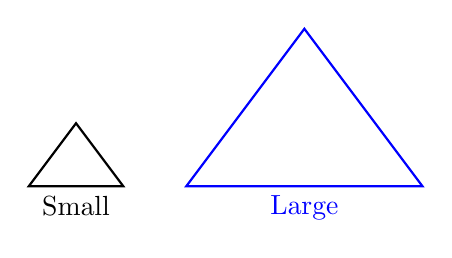
\begin{tikzpicture}[scale=0.4, baseline=(current bounding box.center)]
        % Small Triangle
        \draw[thick] (0,0) -- (3,0) -- (1.5,2) -- cycle;
        \node[below] at (1.5, 0) {Small};
        % Large Triangle
        \draw[thick, blue] (5,0) -- (12.5,0) -- (8.75,5) -- cycle;
        \node[below, blue] at (8.75, 0) {Large};
    \end{tikzpicture}
    \end{center}
    
    \vspace{1.2cm}

    \item \begin{ealglossed}
    A rectangular garden is 10 m long and 6 m wide. A new, similarly shaped garden is to be built. The \ealgloss{area}{pole} of the new garden needs to be 50\ealgloss{\%}{procent} larger than the original.
    \end{ealglossed}
    \begin{enumerate}[label=(\alph*)]
        \item \begin{ealglossed}
        What is the \ealgloss{area}{pole} of the new garden?
        \end{ealglossed}
        \item \begin{ealglossed}
        What is the \ealgloss{perimeter}{obwód} of the new garden?
        \end{ealglossed}
    \end{enumerate}
    \begin{tikzpicture}[baseline=(current bounding box.center)]
        \draw (0,0) rectangle (5, 3);
        \node[above] at (2.5, 3) {10 m};
        \node[right] at (5, 1.5) {6 m};
        \node at (2.5, -0.5) {Original Garden};
    \end{tikzpicture}
    \vspace{1.2cm}
\end{enumerate}


\begin{ealglossed}
\section*{\ealgloss{Rates of Change}{tempo zmian} Past}
\end{ealglossed}

\begin{enumerate}[resume]

    \item \begin{ealglossed}
    A plant was \SI{20}{\centi\meter} tall. Over the next week, it grew by \textbf{5\ealgloss{\%}{procent}}. At what speed did it grow, in cm per day?
    \end{ealglossed}
    \vspace{0.6cm}

    \item \begin{ealglossed}
    A bathtub fills at a \ealgloss{rate}{wielkość ilorazowa} of \SI{8}{\litre\per\minute}. The plug is slightly loose, and water drains out at a \ealgloss{rate}{wielkość ilorazowa} that is 2\ealgloss{\%}{procent} of the fill \ealgloss{rate}{wielkość ilorazowa}. If the tub starts empty, how much water is in it after 10 minutes?
    \end{ealglossed}
    \vspace{0.6cm}

    \item \begin{ealglossed}
    A car's value was \pounds 15,000. It \ealgloss{depreciates}{amortyzacja} (loses value) at a \ealgloss{rate}{wielkość ilorazowa} of 12\ealgloss{\%}{procent} per year. A motorbike's value was \pounds 8,000 and it \ealgloss{depreciates}{amortyzacja} at 8\ealgloss{\%}{procent} per year. After 3 years, which vehicle is worth more? Justify your answer with calculations.
    \end{ealglossed}
    \vspace{0.6cm}

    \item \begin{ealglossed}
    A social media post is shared rapidly. On the first day, it gets 200 shares. The number of shares increases by 15\ealgloss{\%}{procent} each day after that.
    \end{ealglossed}
    \begin{enumerate}
        \item How many shares does it get on the third day?
        \item What is the total number of shares at the end of the third day?
    \end{enumerate}
    \vspace{0.6cm}

    \item \begin{ealglossed}
    A factory's energy costs are \pounds 10,000 per month. The manager invests in new equipment which is 20\ealgloss{\%}{procent} more efficient. However, due to increased production, the factory now runs for 15\ealgloss{\%}{procent} more hours each month, up from 200 hours. Calculate the new energy cost per hour, and per month, assuming cost is \ealgloss{directly proportional}{wprost proporcjonalny} to running hours.
    \end{ealglossed}

\end{enumerate}

\begin{ealglossed}
\section*{\ealgloss{Rates of Change}{tempo zmian} Future}
\end{ealglossed}

\begin{enumerate}[resume]

    \item \begin{ealglossed}
    A \ealgloss{square}{kwadrat} has a side length that is increasing at a \ealgloss{rate}{wielkość ilorazowa} of \SI{2}{\centi\meter\per\second}. What is the \ealgloss{rate of change}{tempo zmian} of its \ealgloss{perimeter}{obwód} when the side length is \SI{5}{\centi\meter}?, what about when the side length is \SI{10}{\centi\meter}? Does the \ealgloss{rate}{wielkość ilorazowa} depend on the side length?
    \end{ealglossed}
    \vspace{0.6cm}

    \item \begin{ealglossed}
    A rectangular car park is \SI{60}{\metre} long and \SI{40}{\metre} wide. It is to be resurfaced. The cost of resurfacing is \pounds 15 per \ealgloss{square}{kwadratowy} metre. Calculate the total cost.
    \end{ealglossed}
    \vspace{0.6cm}

    \item \begin{ealglossed}
    A circular oil spill is spreading. It starts with a \ealgloss{radius}{promień} of 1m. The \ealgloss{radius}{promień} of the spill is increasing at a \ealgloss{constant}{stała} \ealgloss{rate}{wielkość ilorazowa} of \SI{0.5}{\metre\per\minute}.
    \end{ealglossed}
    \begin{enumerate}
        \item \begin{ealglossed}
        Calculate the \ealgloss{rate}{wielkość ilorazowa} at which the \textbf{\ealgloss{circumference}{obwód}} of the spill is increasing when the \ealgloss{radius}{promień} is \SI{4}{\metre}. (Use $C = \pi D$)
        \end{ealglossed}
        \item \begin{ealglossed}
        Calculate the \ealgloss{rate}{wielkość ilorazowa} at which the \textbf{\ealgloss{circumference}{obwód}} of the spill is increasing when the \ealgloss{radius}{promień} is \SI{8}{\metre}.
        \end{ealglossed}
        \item \begin{ealglossed}
        Find the \ealgloss{area}{pole} of the spill after 10 minutes.  (Use $A = \pi r^2$)
        \end{ealglossed}
    \end{enumerate}
    \vspace{0.6cm}

    \item \begin{ealglossed}
    A gardener is planting a rectangular flower bed. The length of the bed is increasing at a \ealgloss{rate}{wielkość ilorazowa} of \SI{1}{\metre\per\hour} and the width is increasing at a \ealgloss{rate}{wielkość ilorazowa} of \SI{0.5}{\metre\per\hour}. At a specific moment, the length is \SI{6}{\metre} and the width is \SI{4}{\metre}.
    \end{ealglossed}
    \begin{enumerate}
        \item \begin{ealglossed}
        At what \ealgloss{rate}{wielkość ilorazowa} is the \textbf{\ealgloss{perimeter}{obwód}} increasing at this moment?
        \end{ealglossed}
        \item \begin{ealglossed}
        How much will the \textbf{\ealgloss{area}{pole}} have increased by 30 minutes later? Do you think it grew at a \ealgloss{constant}{stała} \ealgloss{rate}{wielkość ilorazowa}?
        \end{ealglossed}
    \end{enumerate}
    \vspace{0.6cm}

    \item \begin{ealglossed}
    A decorative path is being built around a rectangular pond. The pond is \SI{10}{\metre} long and \SI{6}{\metre} wide. The path has a \ealgloss{uniform}{jednostajna} width of $x$ metres all the way around.
    \end{ealglossed}
    \begin{enumerate}
        \item \begin{ealglossed}
        Show that the \ealgloss{area}{pole} of the path, $A$, is given by the \ealgloss{formula}{wzór} $A = 4x^2 + 32x$.
        \end{ealglossed}
        \item \begin{ealglossed}
        If the path is being paved at a \ealgloss{rate}{wielkość ilorazowa} of \SI{0.8}{\square\metre\per\minute}, how wide is the path after 20 minutes, assuming it is being paved outwards from the \ealgloss{rectangle}{prostokąt}?
        \end{ealglossed}
    \end{enumerate}

\end{enumerate}

\end{document}